\section{概述}  % Article style
%\chapter{Introduction}  % Report style
\subsection{系统概览}
单目相机和低成本IMU构成了能对空间六自由度状态进行估计的最小传感器单元——惯性视觉导航系统(Visual Inertial Navigation System,VINS)。但距离和位姿直接量测信息的缺乏,给VINS带来了IMU处理、估计器初始化、相机标定和非线性优化等方面的挑战。本文提出了一种鲁棒多功能单目视觉惯性导航系统——VINS-Mono。本方法基于鲁棒初始化和故障恢复,融合紧耦合非线性优化方法、IMU预积分方法以及特征检测方法以获取高精度的视觉惯性里程计。回环检测模块的加入则进一步实现了紧耦合下最小计算量的重定位。此外,本方法还是用四方向位姿图优化加强全局一致性。算法的性能在公开数据集和实际飞行试验中得到了有效验证,并和现有算法进行了对比。
% Following sections, subsections, etc.
% -------------------------------------
单目相机的小尺寸、低成本、易配置等特点使其成为了SLAM领域的最常用传感器,但纯单目视觉系统无法恢复几何尺度;而IMU可以提供几何尺度、角速度等全面的量测信息,同时缓解由于光照变化、特征缺失、运动模糊等带来的视觉跟踪丢失问题。由于单目VINS需要加速度激励才能使几何尺度可观,单目VINS必须在未知的运动而非静止状态下完成初始化,这就给VINS中状态估计器的初始化带来了挑战。

VINS-Mono正是为解决这一问题而诞生,本方法起始于状态估计器的\textbf{在线初始化},核心是基于\textbf{非线性滑窗优化}的\textbf{紧耦合}VIO。该VIO模块不仅提供精确的局部位姿、速度和航向估计,还提供相机-IMU内参和零偏的\textbf{在线修正}。回环检测则基于\textbf{Dow2}词袋实现。重定位基于单目VIO的\textbf{特征级融合}实现以实现最小计算复核下的精确鲁棒回环检测。同时VINS-Mono还加入了\textbf{几何回环}验证模块基于IMU的角度量测优化\textbf{4自由度位姿图}以保证全局一致性。

图\ref{fig.1}给出了VINS的总体结构,系统起始于量测处理模块,包括图像特征的提取和跟踪,以及两图像之间IMU的预积分。随后初始化模块提供位姿、速度、重力矢量、陀螺偏差、3D特征位置等必要的信息供后续基于非线性优化的VIO使用。带有重定位功能的紧耦合VIO模块负责融合预积分的IMU量测、图像特征量测以及回环中重新检测到的图像特征信息。最终,位子图优化基于几何验证重定位结果执行全局优化以消除飘逸。VIO、重定位和位姿图优化分别运行在独立的线程中以保证系统运行的可靠性和实时性。
\subsection{符号约定}
这里首先给出本文中的符号约定。$a$等小写常规字母表示标量,$\bm{x}$等小写加粗字母表示矢量,$\bm{J}$等大写加粗字母表示矩阵。字母上标表示该标量所在的坐标系,$\left(\cdot\right)^w$为世界坐标系,采用N-E-D定义,$z$轴指向重力矢量方向;$\left(\cdot\right)^b$为本体坐标系,采用前右下定义,IMU测量坐标系于本体系一致;$\left(\cdot\right)^w$为相机坐标系,同样采用前右下定义,不同之处在于此处以相机光轴为前。坐标旋转分别采用旋转矩阵$\bm{R}$和四元数$\bm{q}$表示,旋转方向为下标到上标,即$\bm{q}_b^w$表示本体系到世界系的坐标旋转四元数。$\bm{t}_b^w$表示本体系到世界系的坐标平移变换矢量。下标$k$表示当前对应的图像帧,例如$c_k$、$b_k$分别表示第$k$帧图像采集时的本体坐标系和相机坐标系。$\bm{g}=\left[0,0,g\right]^T$为重力矢量。$\otimes$为四元数乘法运算符。使用上标$\hat{\left(\cdot\right)}$表示变量的估计值或测量值,以和实际值区分。

\begin{figure}[htbp]
	\centering
	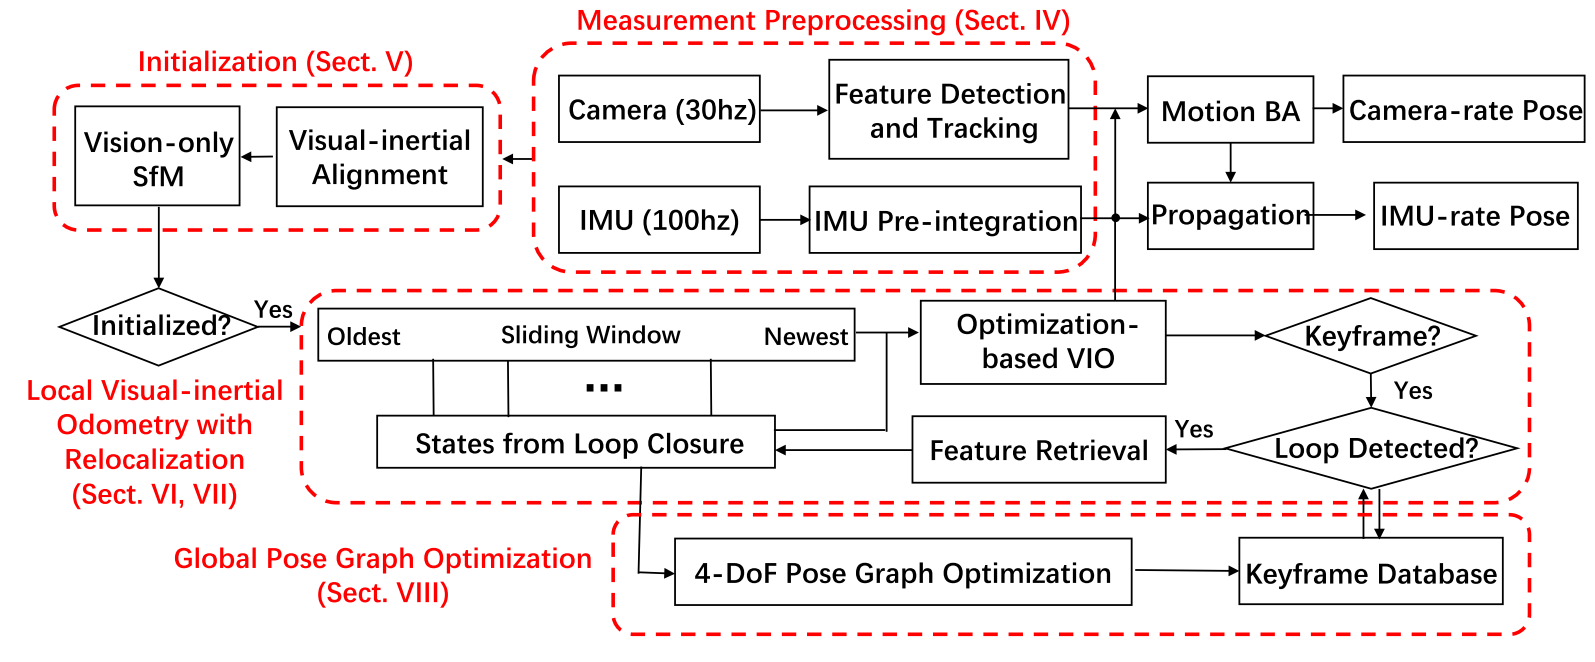
\includegraphics[scale=0.3]{VINS_structure.png}
	\caption{VINS-Mono系统框架}
	\label{fig.1}
\end{figure}      

\section{量测处理}
本节主要介绍连续两帧间IMU和相机的量测处理过程。相机量测处理分为跟踪参考帧关键点(Keypoints)在当前帧中的位置和探测当前帧中新的关键点两部分;IMU量测的处理则主要是在集中在预积分过程。由于低成本IMU中零偏和噪声量级较为接近,这里假设噪声为高斯白噪声,在预积分过程中只考虑器件零偏的影响。
\subsection{视觉前端处理}
对于每一帧新图像,基于KLT稀疏光流法跟踪现有特征;同时采用Shi-Tomasi角点检测检测当前帧中新出现的特征以保证图像中的最小特征数(100-300)。同时,通过设置相邻特征之间的最小像素距离保证特征在图像中均匀分布。2D特征首先经过去畸变处理,随后基于RANSAC算法去除野值量测,最后投影到单位球上。

关键帧的选取则基于以下两个原则。首先,判断两帧之间的平均视差,如果所跟踪的特征在当前帧和上一个参考帧之间的视差超过一定阈值,则将当前帧作为新的关键帧;同时为了分离纯旋转引起的视差变化,对两帧之间的陀螺量测进行积分,补偿旋转的影响。这一旋转补偿只作用于关键帧选取而给位姿估计,因此不会影响位姿估计质量。其次,判断所跟踪的特征数目,若小于一定数量,则将当前帧作为新的关键帧,以防跟踪丢失。
\subsection{IMU预积分}
IMU预积分基于连续时间四元数微分方法实现,相关公式的详细推导参见附录\ref{append.b},这里直接给出结论。
\subsubsection{IMU器件模型}
IMU的量测模型可表示为:
\begin{equation}
\left\{
\begin{aligned}
&\hat{\bm{a}}^b=\bm{a}^b+\bm{b}_a+\bm{R}_w^b\bm{g}^w+\bm{n}_a\\
&\hat{\bm{\omega}}^b=\bm{\omega}^b+\bm{b}_\omega+\bm{n}_\omega
\end{aligned}
\right.
\end{equation}
式中,$\hat{\bm{a}}^b$和$\hat{\bm{\omega}}^b$分别表示IMU的加速度和角速度测量信息;$\bm{a}^b$和$\bm{\omega}^b$分别为载体真实的加速度和角速度;$\bm{b}_a$和$\bm{b}_\omega$分别为加速度计和陀螺仪零偏,建模为随机游走过程:
\begin{equation}
\centering
\left\{
\begin{aligned}
&\bm{n}_{\bm{b}_a}\sim\mathcal{N}\left(\bm{0},\bm{\sigma}_{b_a}^2\right),\bm{n}_{\bm{b}_\omega}\sim\mathcal{N}\left(\bm{0},\bm{\sigma}_{b_\omega}^2\right)\\
&\dot{\bm{b}_a}=\bm{n}_{\bm{b}_a},dot{\bm{b}_\omega}=\bm{n}_{\bm{b}_\omega}
\end{aligned}
\right.
\end{equation}
$\bm{R}_w^b$为世界坐标系到本体坐标系的坐标旋转矩阵;$\bm{g}^w$为世界坐标系下的重力加速度矢量;$\bm{n}_a\sim\mathcal{N}\left(\bm{0},\bm{\sigma}_a^2\right)$和$\bm{n}_\omega\sim\left(\bm{0},\bm{\sigma}_\omega^2\right)$为器件的高斯白噪声。
\subsubsection{IMU预积分项}
由于IMU直接预积分项包含$k$时刻的位姿信息,不便于后端优化,因此使用增量形式的预积分项表达式:
\begin{equation}
\centering
\left\{
\begin{aligned}
&\hat{\bm{\alpha}}_{k+1}^{b_k}=\iint_{t_i\in\left[t_k,t_{k+1}\right]}\left(\bm{R}_{b_{t_i}}^w\left(\hat{\bm{a}}_{t_i}-\bm{b}_a-\bm{n}_a\right)\right)dt^2\\
&\hat{\bm{\beta}}_{k+1}^{b_k}=\int_{t_i\in\left[t_k,t_{k+1}\right]}\left(\bm{R}_{b_{t_i}}^w\left(\hat{\bm{a}}_{t_i}-\bm{b}_a-\bm{n}_a\right)\right)dt\\
&\hat{\bm{\gamma}}_{k+1}^{b_k}=\int_{t_i\in\left[t_k,t_{k+1}\right]}\frac{1}{2}\bm{\Omega}\left(\hat{\bm{\omega}}_{wb}^w-\bm{b}_\omega-\bm{n}_\omega\right)\bm{\gamma}_k^{t_i}dt
\end{aligned}
\right.
\end{equation}
式中$\bm{\alpha}$、$\bm{\beta}$和$\bm{\gamma}$分别为位置、速度和四元数的增量预积分项。
\subsubsection{增量预积分关于零偏的更新}
虽然增量形式的预积分避免了每次后端优化引起$k$时刻位姿变化时都需要重新预积分的问题,但仍需要根据零偏优化数的变化进行更新。为减少计算量,VINS-Mono采取入夏更新策略:当后端优化的IMU零偏变化时,若变化较小,则使用IMU预积分项关于零偏的一阶近似更新预积分项;否则,则按照式\ref{eq.append.b.21}重新积分IMU得到预积分项。IMU预积分关于零偏的线性化更新表达式可以表示为:
\begin{equation}
\left\{
\begin{aligned}
&\hat{\bm{\alpha}}_k^{k+1}\approx\hat{\bm{\alpha}}_k^{k+1}+\bm{J}^{\bm{\alpha}}_{\bm{b}_a}\delta\bm{b}_a+\bm{J}^{\bm{\alpha}}_{\bm{b}_\omega}\delta\bm{b}_\omega\\
&\hat{\bm{\beta}}_k^{k+1}\approx\hat{\bm{\beta}}_k^{k+1}+\bm{J}^{\bm{\beta}}_{\bm{b}_a}\delta\bm{b}_a+\bm{J}^{\bm{\beta}}_{\bm{b}_\omega}\delta\bm{b}_\omega\\
&\hat{\bm{\gamma}}_k^{k+1}=\hat{\bm{\gamma}}_k^{k+1}\otimes\bm{J}^{\bm{\gamma}}_{\bm{b}_\omega}\delta\bm{b}_\omega
\end{aligned}
\right.
\label{eq.2.4}
\end{equation}
\section{估计器初始化}
单目紧耦合VIO是一个高度依赖于精确初始值的非线性系统,VINS-Mono通过IMU预积分和视觉SfM(Structure from Motion)获得的松耦合对准获得。
\subsection{相机与IMU外参对准}
与精确标定的数据集不同,在一些实际应用中,相机和IMU之间外参矩阵的标定精度不够。对于这种情况,VINS-Mono将标定后的外参作为初值,在初始化过程中对其进行进一步优化。由于平移的影响并没有旋转显著,VINS-Mono只考虑IMU与相机之间相对旋转矩阵的标定。

假设相机得到的两帧之间旋转矩阵为$\bm{R}_{c_k}^{c_{k+1}}$,IMU预积分得到的旋转矩阵为$\bm{R}_{b_k}^{b_{k+1}}$,相机和IMU之间的旋转矩阵为$\bm{R}_b^c$,则对于任意两帧图像,均有:
\begin{equation}
\bm{R}_{b_{k+1}}^{b_k}\bm{R^b_c}=\bm{R}_c^b\bm{R}_{c_{k+1}}^{c_k}
\end{equation}
\subsection{滑窗内的纯视觉SfM}
\subsubsection{算法概览}
为了限制算法的计算规模,前端在滑动窗口内仅维持有限数目的图像帧。首先,检测最后一帧图像和窗口内所有其他图像中的特征跟踪情况:若最后一帧图像和任意一个图像帧的稳定跟踪特征超过30个(\textit{程序中设定是15对,这里概念不是很清楚}),且有效视差超过20对,则基于五点法恢复两帧之间的位姿。随后基于五点法恢复的位姿,对这两帧中跟踪到的特征点进行三角化,再基于三角化后的特征点利用PnP算法估计所有帧位姿,最终基于全局BA算法最小化所有特征点的总重投影误差。(这里原文说明的流程并不清楚,究竟是哪些帧之间的位姿,哪一帧向哪一帧的重投影误差,需要进一步参考程序。)由于纯视觉系统缺乏有关世界坐标系的先验信息,这里假设第一帧的相机坐标系(此处是否指的是窗口内的第一帧?)为参考坐标系,所有的相机位姿$\left(\overline{\bm{p}}_{c_k}^{c_0},\bm{q}_{c_k}^{c_0}\right)$和特征点位置均表示在第一帧坐标系下。记相机和IMU之间的外参为$\left(\bm{p}_c^b,\bm{q}_c^b\right)$,则IMU坐标系在$c_0$下的位姿为:
\begin{equation}\begin{aligned}
&\bm{q}_{b_k}^{c_0}=\bm{q}_b^c\otimes\bm{q}_{c_k}^{c_0}\\
&s\overline{\bm{p}}_{b_k}^{c_0}=s\overline{p}_{c_k}^{c_0}-\bm{p}^c_b
\end{aligned}
\end{equation}
\subsubsection{程序解析}
滑窗内的纯视觉SfM包含在GlobalSFM类中,对应头文件和源文件为vins\_estimator/initial文件夹下的initial\_sfm.cpp和initial\_sfm.h,该类只有唯一的一个公共借口函数constructor(),对应的算法流程如下:
\begin{enumerate}
	\item 选取包含$k$个图像帧的滑动窗口,将窗口内的第1帧图像对应的位姿设为基准位姿,记该图像的序号为$l$;利用对极几何约束(五点法或八点法)恢复第$k$帧的相对位姿;
	\item 基于第1帧和第$k$帧的位姿三角化部分特征点的空间位置信息;
	\item 从已三角化的特征点集合中选取能被第2帧图像看到的特征点,基于PnP求解第2帧的相对位姿;
	\item 基于第一帧和第$k$帧的位姿三角化部分特征点的空间位置信息,第2步中已经三角化的特征点会被直接跳过;
	\item 重复上述步骤直到第$k-1$帧,此时滑窗内所有图像帧相对于第1帧的相对位姿均已获得。
	\item 依次基于第1帧位姿和第$i$帧位姿三角化前序过程中剩余的特征点;
	\item 基于现有的特征点空间信息,利用PnP求解窗口内第$l-1$帧图像的相对位姿;
	\item 基于第$l$帧和第$l-1$帧位姿三角化部分特征点的空间信息;
	\item 重复7、8两步直到系统起始时刻的第0帧图像;
	\item 至此,所有图像帧的相对位姿均解算完毕,对于此时仍未三角化的特征点,选择其第一次和最后一次被观测到的图像帧,进行三角化。
	\item 使用Ceres对现有所有图像帧的位姿和空间点的三维坐标进行BA优化。
	
\end{enumerate}
\subsection{惯性视觉对准}
惯性视觉对准的基本思想是将IMU的与积分值与视觉SfM获得了待尺度的数值进行匹配。
\subsubsection{陀螺零偏标定}
考虑窗口内的连续两帧$\bm{b}_k$和$\bm{b}_{k+1}$,我们已经通过纯视觉SfM计算出了对应的旋转$\bm{q}_{b_k}^{c_0}$和$\bm{q}_{b_{k+1}}^{c_0}$,同时IMU预积分也提供了$k$帧到$k+1$帧的相对姿态约束$\bm{\gamma}^{b_k}_{k+1}$,通过最小化两者之间的误差来实现IMU和视觉量测的对准:
\begin{equation}
\min\limits_{\delta\bm{b}_\omega}\sum\limits_{k\in\mathcal{B}}\|\bm{q}_{b_{k+1}}^{c_0}\otimes{\bm{q}_{b_k}^{c_0}}^{-1}\otimes\bm{\gamma}^{b_k}_{k+1}\|^2
\end{equation}
将式\ref{eq.2.4}中的IMU预积分关于陀螺零偏的线性形式带入,则可通过非线性优化方式得到对陀螺零偏的最优估计,再利用新获得的陀螺零偏更新IMU的预积分项。
\subsubsection{速度矢量、重力矢量及几何尺度初始化}
